\section{Notation}
\par $I, X, Y, Z$are the pauli matrices like below.
$$I=
\begin{pmatrix}
1 & 0\\
0 & 1\\
\end{pmatrix}$$
$$X=
\begin{pmatrix}
0 & 1\\
1 & 0\\
\end{pmatrix}$$
$$Y=
\begin{pmatrix}
0 & -i\\
i & 0\\
\end{pmatrix}$$
$$Z=
\begin{pmatrix}
1 & 0\\
0 & -1\\
\end{pmatrix}$$
\par Rotation operators $R_x, R_y, R_z$ are 1-qubit parameterized gates. These operators rotate the quantum state when considering the Bloch sphere by $\theta$ (parameter) about $X$ axis, $Y$ axis, $Z$ axis respectively. It is represented as follows using a matrix:

$$R_x(\theta)=\begin{pmatrix}
\cos{\theta} & -i\sin{\theta}\\
-i\sin{\theta} & \cos{\theta}\\
\end{pmatrix}$$

$$R_y(\theta)=\begin{pmatrix}
\cos{\theta} & -\sin{\theta}\\
\sin{\theta} & \cos{\theta}\\
\end{pmatrix}$$
$$R_z(\theta)=\begin{pmatrix}
\exp{\left(-i\frac{\theta}{2}\right)} & 0\\
0 & \exp{\left(i\frac{\theta}{2}\right)}\\
\end{pmatrix}$$

\par $\sqrt{X}$ gate is 1-qubit gate. If this gate is applied twice continuously on the qubit, the result is the same applying the x gate. Expressing this operation using a matrix gives:
$$\sqrt{X}=\frac{1}{2}
\begin{pmatrix}
1+i & 1-i\\
1-i & 1+i\\
\end{pmatrix}$$

\par CZ gate is the 2-qubits gate and works as a phase flipper for the target qubit if the control qubit is in $|1\rangle$. This gate is symmetric, that is, if the controled qubit and the target are exchanged, the result of the obtained quantum state is the same. Expressing this operation using a matrix gives:
$$
\begin{aligned}
CZ&=|0\rangle\langle0|\otimes I+|0\rangle\langle0|\otimes Z\\
&=\begin{pmatrix}
1 & 0 & 0 & 0\\
0 & 1 & 0 & 0\\
0 & 0 & 1 & 0\\
0 & 0 & 0 & -1\\
\end{pmatrix}
\end{aligned}$$

\begin{figure}[H]
    \centering
    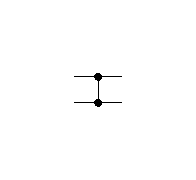
\includegraphics[keepaspectratio, scale=4]{preliminary/CZ.pdf}
    \caption{CZ gate is represented in the picture of quantum circuit like above.}
    \label{fig:CZ}
\end{figure}

\par Assume the $2\times 2$ unitary matrix $U$. When this matrix operation is applied to the $i$-th qubit of the circuit with $Q$ qubits, then $U_d$ is the unitary operation for circuit where the operation $U$ is applied to the $(d \mod Q)$-th qubit, and do nothing to any other qubits. Written as a formula, it looks like this:
$$U_d = I^{\otimes (e-1)}\otimes U\otimes I^{\otimes (Q-e)}$$
where
$$e = d\mod Q$$